\documentclass[en,hazy,blue,screen,14pt]{elegantnote}
\usepackage[T1]{fontenc}
\usepackage[latin9]{inputenc}
\usepackage{babel}
\usepackage{float}
\usepackage{textcomp}
\usepackage{amsmath,amsfonts,amssymb}
\usepackage{amsthm}
\usepackage{graphicx}
\usepackage[ruled,vlined]{algorithm2e}
\PassOptionsToPackage{normalem}{ulem}
\usepackage{ulem}
\usepackage{mathtools}
\DeclarePairedDelimiter{\ceil}{\lceil}{\rceil}

\title{Class Notes\\CIS 502 Analysis of Algorihtm}
\author{Da Kuang}
\institute{University of Pennsylvania}
% \version{1.00}
\date{}

\begin{document}

\maketitle
\newpage
\part{Algorithm Basics}

\section{Introduction}

First, let's talk about cases. A case of input for an algorithm is
associated with an instance of a problem. For the sorting problem
(where we want to find a permutation of a set in a specific order),
I can look at an instance like the set of numbers \{1, 5, 4, 2, 6\}.
This set of numbers would be the input to a sorting algorithm that
purports to solve the sorting problem, like Selection Sort, or one
of the other sorting algorithms out there. 

The same sets of inputs can be given to any algorithm that wants to
solve a problem. It doesn't matter what sorting algorithm I use, the
set of inputs is always the same (because, by definition, they're
all instances of the same problem). However, a given case can be better
or worse for a given algorithm. Some algorithms always perform the
same no matter what the inputs are, but some algorithms might do worse
on some inputs. However, this means that every algorithm has some
best case and some worst case; we also sometimes talk about the average
case (by taking the average of all the cases) or the expected case
(when we have some reason to expect that one case will be more common
than others).

% 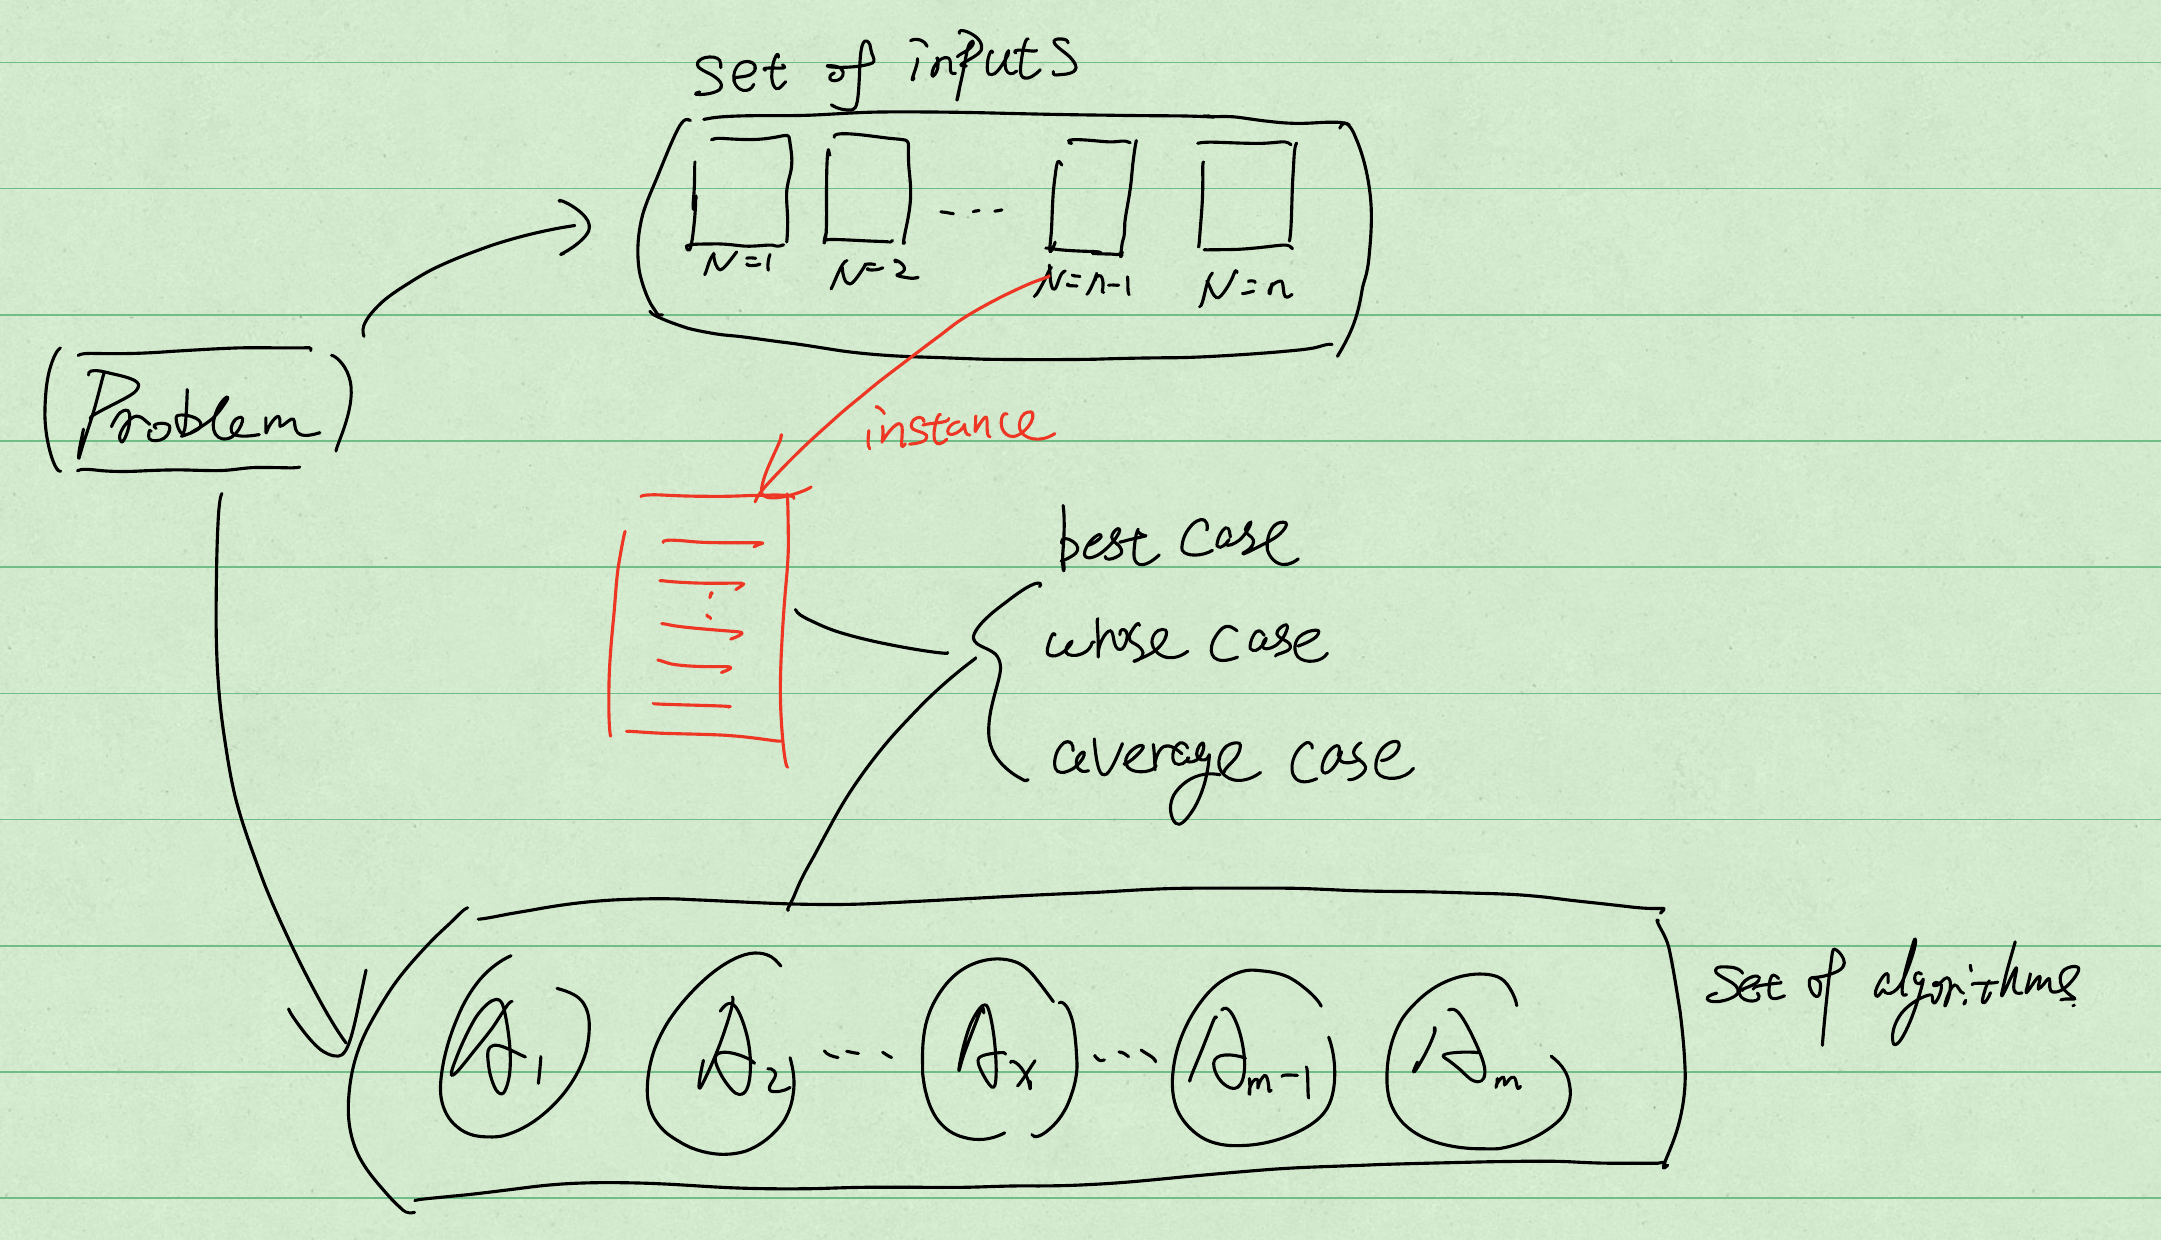
\includegraphics{inputs-algorithm-cases}

\subsection{Algorithm Case Examples }

The problem of \textquotedbl find the minimum of an unsorted list\textquotedbl{}
always works the same for every possible input. No matter what clever
algorithm you write, you have to check every element. It doesn't matter
if you have a list of zeros or a list of random numbers or a list
where the first element is the minimum, you don't know until you get
to the end. Every case is the same for that algorithm, so the best
case is the worst case, and also the average case and the expected
case. If the list was sorted, we could do better, but that's a different
problem.

The problem of \textquotedbl find a given element in a list\textquotedbl{}
is different. Assuming you were using an algorithm that does a linear
walk through the list, it might turn out that the given element was
the first element of the list and you're done immediately. However,
it might also be the last element of the list, in which case you have
to walk the whole thing before you find it. So there you had a best
case and a worst case.

\subsection{Algorithms as Functions of Input Size}

When we want to analyze an algorithm, us algorists think about every
possible case we could throw at the algorithm. Usually, the two most
interesting cases are the best case and the worst case. If you think
of the algorithms runtime as a function of its input, the best case
is the input that minimizes the function and the worst case is the
input that maximizes the function. I'm using \textquotedbl function\textquotedbl{}
in the Algebra math sense here: a series of x/y pairs (input/output
pairs, or in this case \textquotedbl input size/number of execution
steps\textquotedbl ) that draw a line.

Because algorithms' run-time is a function of its input, we have a
different best case (and worst case) for each possible input size.
So sometimes we treat the best case as a single input, but it's really
a set of inputs (one for each input size). The best case and worst
case are very concrete things with respect to a given algorithm.

\subsection{Bounds }

\centerline{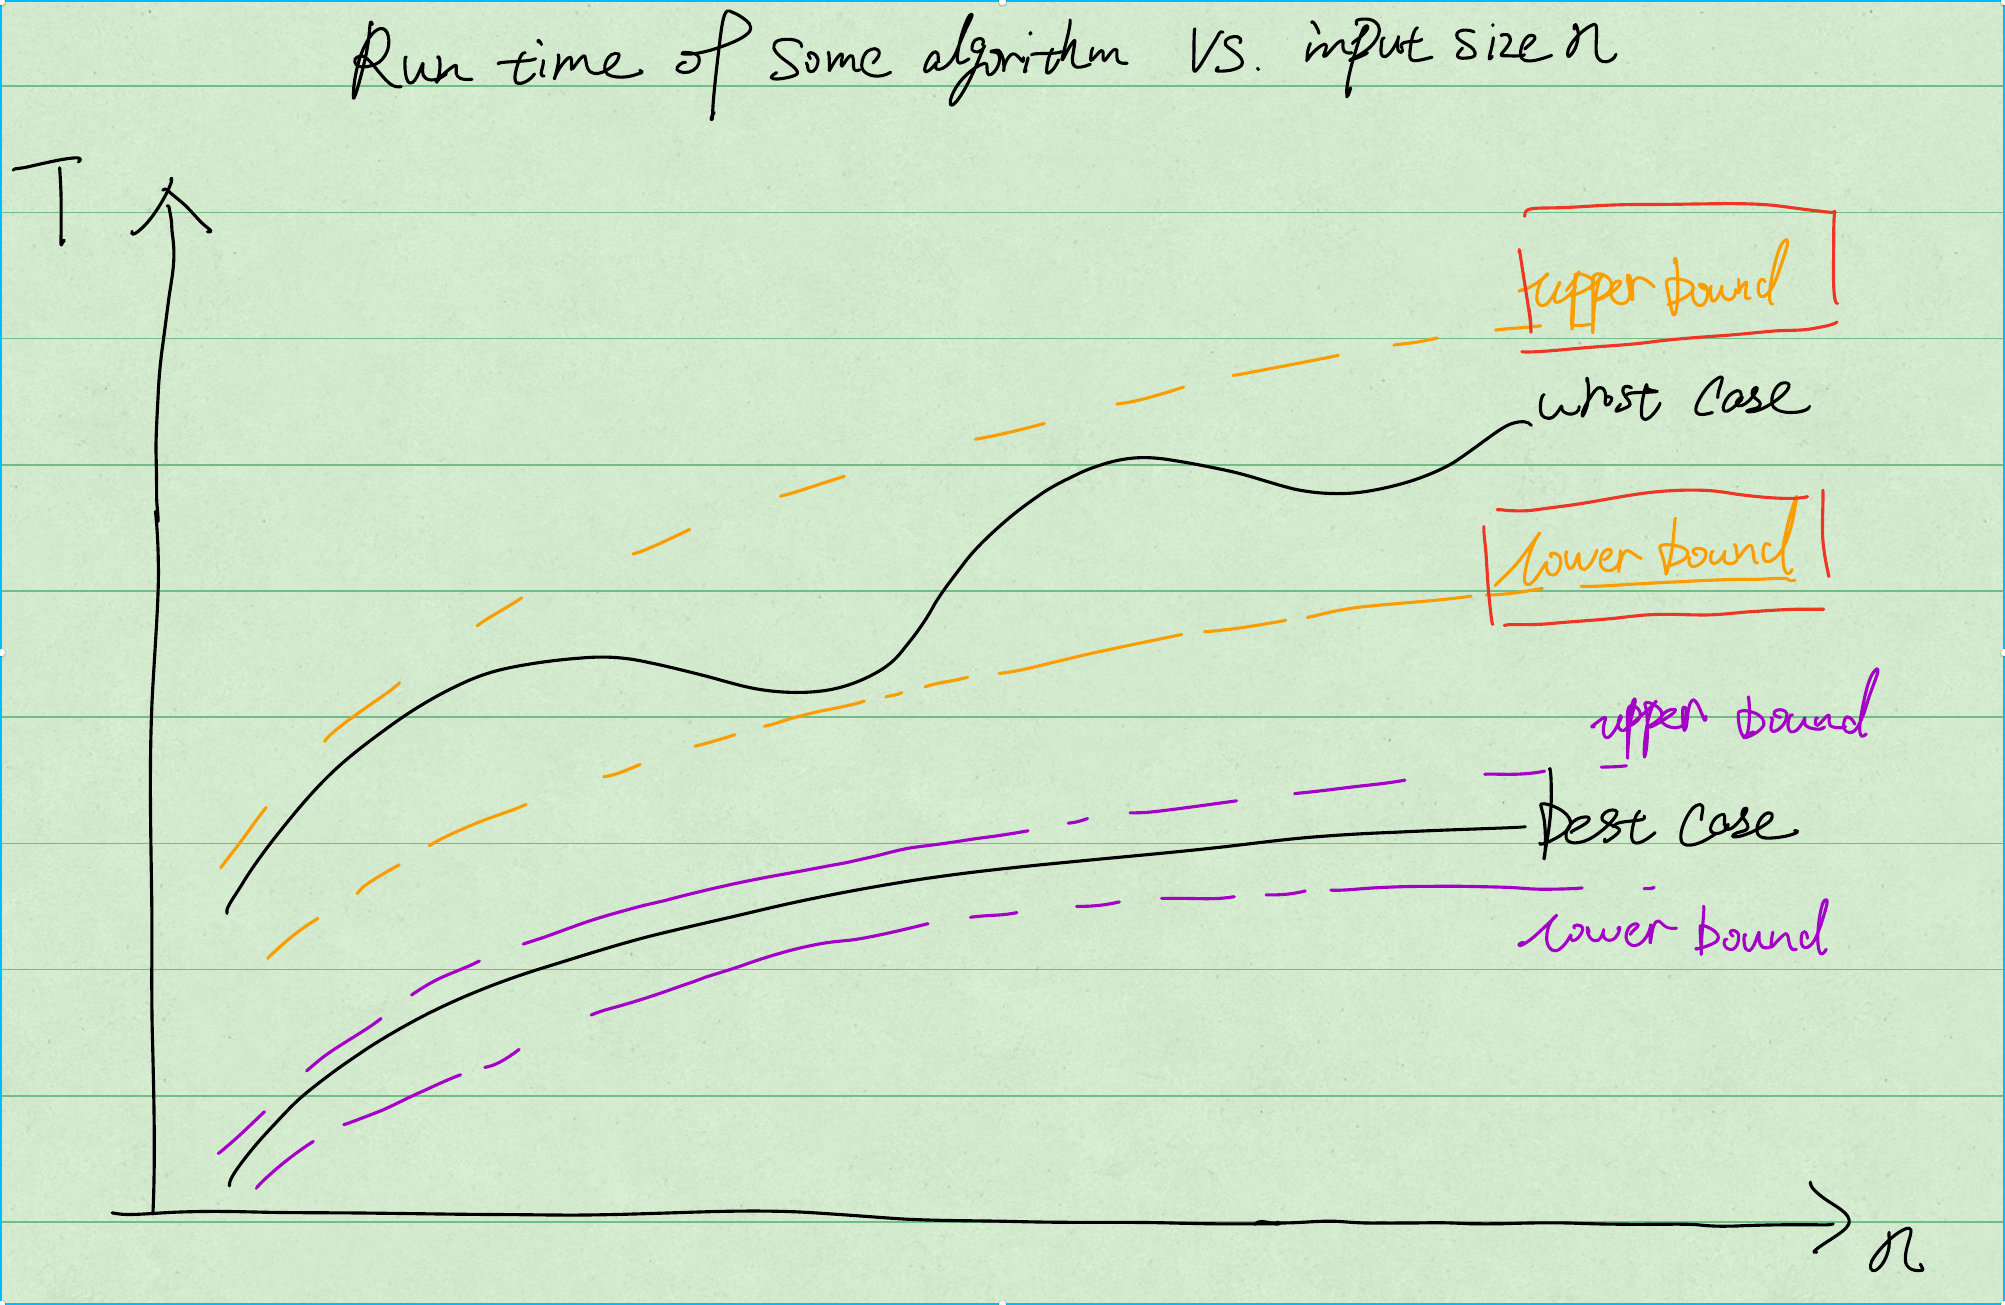
\includegraphics[width=0.6\textwidth]{bounds.png}}

Now what about bounds? Bounds are functions that we use to compare
against a given algorithm's function. There are an infinite number
of boundary functions we could consider. How many possible kinds of
lines can you draw on a graph? That's how many boundary functions
there are. Most algorists are usually only interested in a few specific
functions: things like the constant function, the linear function,
the logarithmic function, the exponential function, etc.

\textbf{An upper bound is a function that sits on top of another function.
A lower bound is a function that sits under the other function.} When
we talk about Big O and Big Omega, we don't care if the bounds are
ALWAYS above or below the other function, just that after a certain
point they always are (because sometimes algorithms get weird for
small input sizes). 

There are an infinite number of possible upper bounds for any given
function, and an infinite number of possible lower bounds for any
given function. But this is one of those weird times when we're talking
about different sizes of infinities. To be an upper bound, the function
must not be below the other function, so we rule out the infinite
number of functions below the other function (so it's smaller than
the set of all possible functions).

Of course, just because there are infinite upper bounds, doesn't mean
they're all useful. The function f(\ensuremath{\infty}) is an upper
bound for every function, but that's like saying \textquotedbl I
have less than an infinite number of dollars\textquotedbl{} - not
particularly useful for figuring out if I'm penniless or a millionaire.
So we are often interested in an upper bound that is \textquotedbl\textbf{tight}\textquotedbl{}
(also known as a \textquotedbl least upper bound\textquotedbl{} or
\textquotedbl supremum\textquotedbl ), for which there is no better
upper bound.

\subsection{Best/Worst Case + Lower/Upper Bound }

We have best/worst cases that represent the upper and lower functions
of an algorithms' runtime function. We have upper and lower bounds
that represent other functions that could be on top or below (respectively)
any other function. They can be combined to articulate key ideas about
algorithms.
\begin{itemize}
\item \textbf{Worst Case Lower Bound}: A function that is a boundary below
the algorithms' runtime function, when that algorithm is given the
inputs that maximize the algorithm's run time.
\item \textbf{Worst Case Upper Bound}: A function that is a boundary above
the algorithms' runtime function, when that algorithm is given the
inputs that maximize the algorithm's run time.
\item \textbf{Best Case Lower Bound}: A function that is a boundary below
the algorithms' runtime function, when that algorithm is given the
inputs that minimize the algorithm's run time.
\item \textbf{Best Case Upper Bound}: A function that is a boundary above
the algorithms' runtime function, when that algorithm is given the
inputs that minimize the algorithm's run time.
\end{itemize}

\subsection{Examples of Case Bounds}

Let's give concrete examples of when we might care about each of these:

\subsubsection*{Worst Case Lower Bound}

The classic example here is comparison-based sorting, which is famously
known to be $\Omega(n\log(n))$ in the worst case. No matter what
algorithm you devise, I can pick a set of worst-case inputs whereby
the tightest lower bound function is log-linear. You cannot make an
algorithm that beats that bound for the worst case, and you shouldn't
bother trying. It's the basement of sorting. Of course, there are
many lower bounds for the worst case: constant, linear, and sub-linear
are all lower bounds. But they are not useful lower bounds, because
there the log-linear lower bound is the tightest one.

\subsubsection*{Best Case Lower Bound}

Insertion Sort works by walking through the list, and inserting any
out-of-order it comes across in the right place. If the list is sorted,
it will only need to walk through the list once without doing any
inserts. This means that the tightest lower bound of the best case
is $\Omega(n)$. You cannot do better than that without sacrificing
correctness, because you still need to be able to walk through the
list (linear time). However, the lower bound for the best case is
better than the lower bound for the worst case!

\subsubsection*{Worst Case Upper Bound}

We are often interested in finding a tight upper bound on the worst
case, because then we know how poorly our algorithm can run in the
worst of times. Insertion sort's worst case is a list that is completely
out of order (i.e. completely reversed from its correct order). Every
time we see a new item, we have to move it to the start of the list,
pushing all subsequent items forward (which is a linear time operation,
and doing it a linear number of times leads to quadratic behavior).
However, we still know that this insertion behavior will be $O(n^{2})$
in the worst case, acting as a tight upper bound for the worst case.
It's not great, but it's better than an upper bound of, say, exponential
or factorial! Of course, those are valid upper bounds for the worst
case, but again that's not as useful as knowing that quadratic is
a tight upper bound.

\subsubsection*{Best Case Upper Bound}

What's the worst our algorithm can do in the best of times? In example
before of finding an element in a list, where the first element was
our desired element, the upper bound is O(1). In the worst case it
was linear, but in the best case, the worst that can happen is that
it's still constant. This particular idea isn't usually as important
as Worst Case Upper Bound, in my opinion, because \textbf{we're usually
more concerned with dealing with the worst case}, not the best case.

Some of these examples are actually $\Theta$, not just $O$ and $\Omega$.
In other cases, I could have picked lower or upper bound functions
that weren't tight, but were still approximate enough to be useful
(remember, if we're not being tight, I have an infinite well to draw
from!). Note that it can be difficult to find compelling examples
of different case/bound combinations, because the combinations have
different utility.

\subsection{Misconceptions and Terminology} 

Frequently, you'll see people with misconceptions about these definitions.
In fact, many perfectly good Computer Scientists will use these terms
loosely and interchangeably. However, the idea of cases and bounds
ARE distinct, and you would do well to make sure you understand them.
Does this mean the difference will come up in your day-to-day? No.
But when you are choosing between a few different algorithms, you
want to read the fine print about the cases and bounds. \emph{Someone
telling you that their algorithm has a Best Case Upper Bound of O(1)
is probably trying to pull the wool over your eyes - make sure you
ask them what the Worst Case Upper Bound is!}

\subsection{Reference}

\href{https://stackoverflow.com/questions/7628991/upper-bound-vs-lower-bound-for-worst-case-running-time-of-an-algorithm}{Upper bound vs lower bound for worst case running time of an algorithm}

\newpage

\section{The asymptotic efficiency of algorithms}

The order of growth of the running time of an algorithm gives a simple
characterization of the algorithm\textquoteright s efficiency and
also allows us to compare the relative performance of alternative
algorithms. Although we can sometimes determine the exact running
time of an algorithm, the extra precision is not usually worth the
effort of computing it. 

We are studying the asymptotic efficiency of algorithms. That is,
we are concerned with how the running time of an algorithm increases
with the size of the input in the limit, as the size of the input
increases without bound. Usually, an algorithm that is asymptotically
more efficient will be the best choice for all but very small inputs.

\subsection{Asymptotic notation }

In this class, we usually apply asymptotic notation to characterize
the running times of algorithms. Even when we use asymptotic notation
to apply to the running time of an algorithm, we need to understand
which running time we mean. Sometimes we are interested in the \textbf{worst-case
running time}. Often, however, we wish to characterize the running
time no matter what the input. In other words, we often wish to make
\textbf{a blanket statement that covers all inputs, not just the worst
case}. We shall see asymptotic notations that are well suited to characterizing
running times no matter what the input.

\centerline{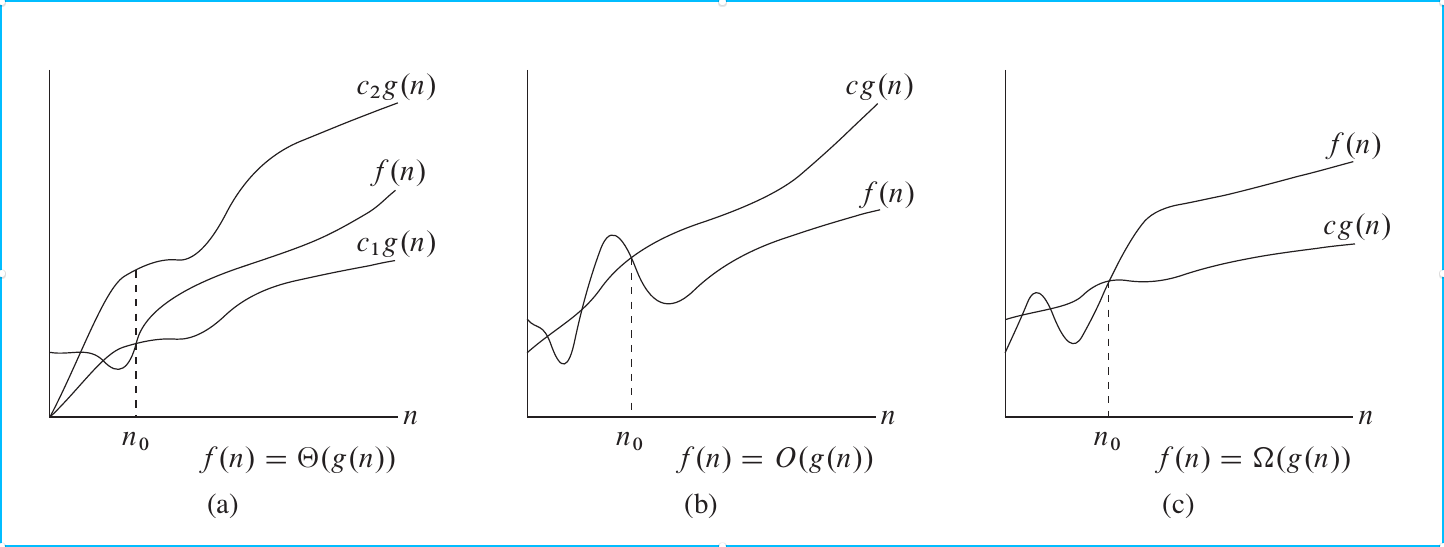
\includegraphics[width=0.7\textwidth]{asymptotic-notion}}

\subsubsection*{$\Theta$-notation}
There exist positive constant $c_{1},c_{2}$ and $n_{0}$ such that,
\[
\Theta(g(n))=\{f(n): 0\le c_{1}g(n)\le f(n)\le c_{2}g(n)\text{ for all 
}n\ge n_{0}\}
\]

$g(n)$ is an asymptotically \textbf{tight bound} for $f(n)$.

\subsubsection*{$O$-notation}
There exist positive constant $c$ and $n_{0}$ such that,
\[
\Theta(g(n))=\{f(n):0\le f(n)\le cg(n)\text{ for all }n\ge n_{0}\}
\]

$g(n)$ is an asymptotic \textbf{upper bound} for $f(n)$.

Using O-notation, we can often describe the running time of an algorithm
merely by inspecting the algorithm\textquoteright s overall structure.
Since O-notation describes an upper bound, when we use it to bound
the worst-case running time of an algorithm, we have a bound on the
running time of the algorithm on every input---the blanket statement
we discussed earlier. 

Notes, when we say ``the running time of insertion sort is $O(n^{2})$'',
we that ``the \textbf{worst-case running time} is $O(n^{2})$''.

\subsubsection*{$\Omega$-notation}

\[
\Omega(g(n))={f(n):\text{there exist positive constant}c\text{and}n_{0}\text{such that}0\le cg(n)\le f(n)\text{ for all }n\ge n_{0}}
\]

$g(n)$ is an asymptotic \textbf{lower bound} for $f(n)$.

When we say that the running time (no modifier) of an algorithm is
$\Omega(g(n))$, we mean that \uwave{no matter what particular
input of size n} is chosen for each value of n, the running time on
that input is at least a constant times $g(n)$, for sufficiently
large n. Equivalently, we are giving a lower bound on \textbf{the
best-case running time} of an algorithm. 

\subsection{Lower Bounds}

Usually in \emph{Algorithm Analysis} we are looking for upper bounds
on cost, as in \textquotedbl Algorithm X solves problem Y in no more
than $O(n^{22/7})$ time in the worst case.\textquotedbl{} Upper bounds
are useful when we want to advertise that our algorithm is good. But
what if \textbf{we want to argue that no other algorithm can be better,
or perhaps that some problem is so hard that we can't possibly hope
to find a good solution to it}?

For this we need a lower bound. Lower bounds come in two flavors:
\begin{itemize}
\item A lower bound on \textbf{an algorithm} is just a \textbf{big-Omega}
bound on its worst-case running time. \textquotedbl I don't know
exactly how long Bogosort takes in general, but I can prove its worst-case
time is $\Omega(n^{2})$.\textquotedbl{}
\item A lower bound on \textbf{a problem} is a \textbf{big-Omega} bound
on the worst-case running time of any algorithm that solves the problem: 
\begin{itemize}
\item \textquotedbl Any comparison-based sorting routine takes $\Omega(n\log n)$
time.\textquotedbl{} 
\item \textquotedbl There is an $\varepsilon>0$ such that any algorithm
for Independent Set takes $\Omega((1+\varepsilon)n)$ time.\textquotedbl{} 
\end{itemize}
\end{itemize}

\subsection{Proving Lower Bounds}

For any computational problem there are many different (often infinitely
many) algorithms that solve the problem. 
\begin{itemize}
\item \textbf{Upper bound of a problem}: To prove $O(f(n))$  for the problem,
we need to show that there is an algorithm that solves the problem
and takes no more than $f(n)$ time on each input of length n.
\item \textbf{Lower bound of a problem}: To prove $\Omega(g(n))$  for
the problem, we need to show that for each algorithm A and for each
(sufficiently large) length n, there is an input on which A takes
at least $g(n)$ time.
\item \textbf{Tight bounds of a problem}: When we can prove lower and upper
bounds for a problem that are the same, then we say that we have tight
bounds.
\end{itemize}
$\textbf{Proofs of lower bounds are often harder}$ since we have to
reason about every possible algorithm to solve the problem. In order
to prove lower bounds, we often have to restrict the power of the
algorithms we consider. This is done by specifying a model of computation,
which lists the primitive operations that an algorithm is allowed
to perform. Most of the lower bounds developed in the literature are
fairly ad hoc but there are a few general techniques that are used.

Why one might want to prove lower bounds:
\begin{itemize}
\item From the \uline{theoretical point of view} we can say that we understand
a computational problem really well if we can prove tight lower and
upper bounds and understanding of these problems is one of the major
goals of computer science. 
\item More \uline{practically}, tells us where to stop in our search
for better and better algorithms for a problem. 
\item The lower bound proof often highlights good and bad strategies for
algorithms to follow and thereby might help in the design of good
algorithms. 
\end{itemize}

\subsubsection*{Information-Theoretic Techniques}

These techniques work in \textbf{restricted models} of computation,
such as the \textbf{comparison tree model}. In this model, an algorithm
is only allowed to perform comparisons between its input elements.
The structure of any such algorithm can be viewed as a tree; hence
the name of the model. 

Each internal node is labeled by a comparison and the two children
of an internal node represent the two possible results of the comparison. 

The leaves represent solutions to the problem. If we can lower bound
the number of possible distinct solutions, this is also a lower bound
on the number of leaves. This in turn translates into a lower bound
on the height of the comparison tree. Since the height of the tree
represents the worst-case number of comparisons performed by the algorithm
we get the desired lower bound. 

\subsubsection*{Potential functions}

This technique for proving lower bounds associates some sort of potential
function that needs to be changed from some initial value to some
final value by the algorithm. If we can show that each step of the
algorithm does not change the potential too much, we can get a lower
bound on the number of steps. 

\subsubsection*{Adversary lower bounds}

One problem that we have with proving lower bounds is that different
algorithms have different worst-cases. Thus we cannot set up one input
and analyze all algorithms on this input and get a good lower bound.
The two techniques we have discussed so far do not create bad inputs
tailored to each algorithm to prove lower bounds. The adversary technique
does. How can we demonstrate a worst-case input for each of a potentially
infinite collection of algorithms? 

The trick is to design a strategy for the adversary that fields questions
made by any algorithm and answers these questions in such a way that
the progress of the algorithm to the solution is slowed down as much
as possible. A strategy for an adversary defines an answer down as
much as possible. A strategy for an adversary defines an answer for
each possible question in each possible \textquoteleft state\textquoteright ,
where a state is the set of questions that have been asked and answers
that have been given to these questions. 

Thus it can be seen that \textbf{the adversary is adaptively creating
a worst-case input for the algorithm}. \textbf{\emph{One constraint
is that the adversary should give a consistent set of answers}}, i.e.,
it should be possible to create an input for which all of the adversary\textquoteright s
answers are correct. An analysis of the adversary\textquoteright s
strategy can then lead to a lower-bound for all comparison-based algorithms
for a problem. 

\emph{Why does worst-case analysis help us to find the lower bound,
which is the best case?}

Looking at the adversary strategy gives us a good idea of how to design
an optimal algorithm for the problem. It provides us with a way to
create worst-case inputs for any algorithm we consider and it also
points to what kinds of comparisons are good to make. 

Example:
\begin{itemize}
\item Finding the Maximum and the Minimum of n elements
\item Merging two sorted lists of length
\begin{itemize}
\item Let $a_{1}<\cdots<a_{n}$ and $b_{1}<\cdots<b_{n}$ be the two lists
of length $n$. When the algorithm compares $a_{i}$ with $b_{j}$,
the adversary answers $a_{i}<b_{j}$ whenever $i\le j$ and $b_{j}<a_{i}$
otherwise.
\item We claim that this strategy ensures that the algorithm must perform
$2n-1$ comparisons. 
\begin{proof}
To prove the claim we make a more specific claim. For $i=1,\cdots,n-1$
the algorithm must compare $b_{i}$ with $a_{i}$ as well as $a_{i+1}$.
Also, the algorithm must compare $b_{n}$ with $a_{n}$.

The aim of the adversary is to make the merging algorithm running
as slow as possible. The given adversary strategy makes two interleaving
ascending arrays and makes sure that $b_{i}$ is only able to be placed
before or after $a_{i}$ such which slows down the merging procedure.
Given this adversary strategy, even for the best/simplest algorithm,
it still cost $2n-1$ steps to merge two list. 

% 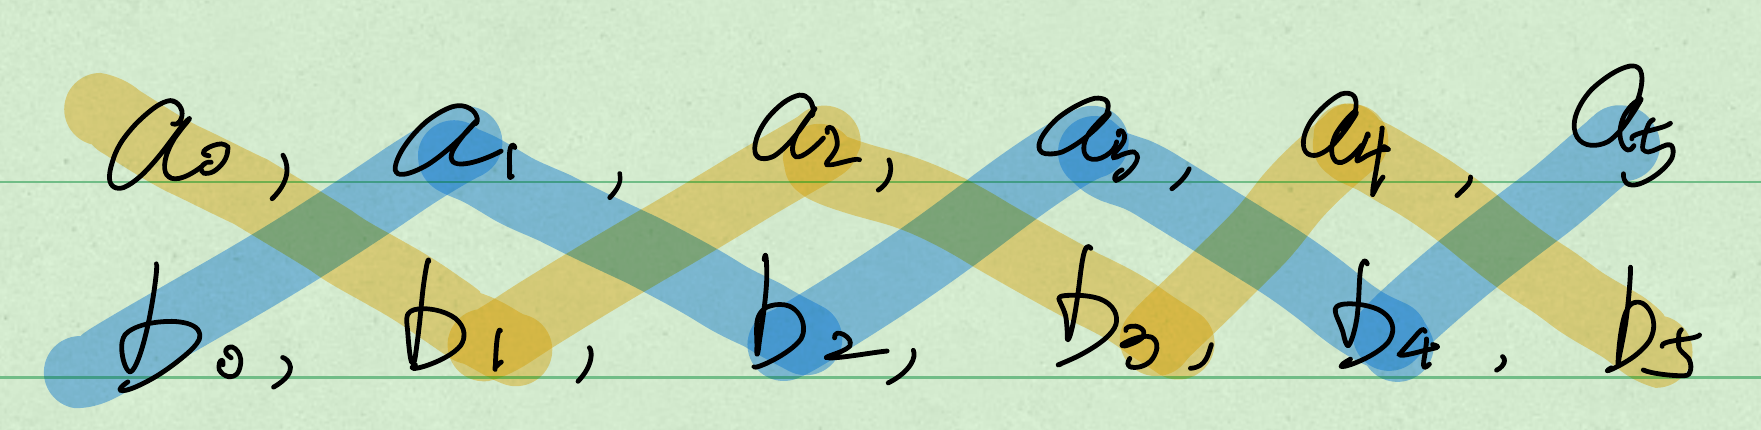
\includegraphics{merging-two-sorted-lists}
\centerline{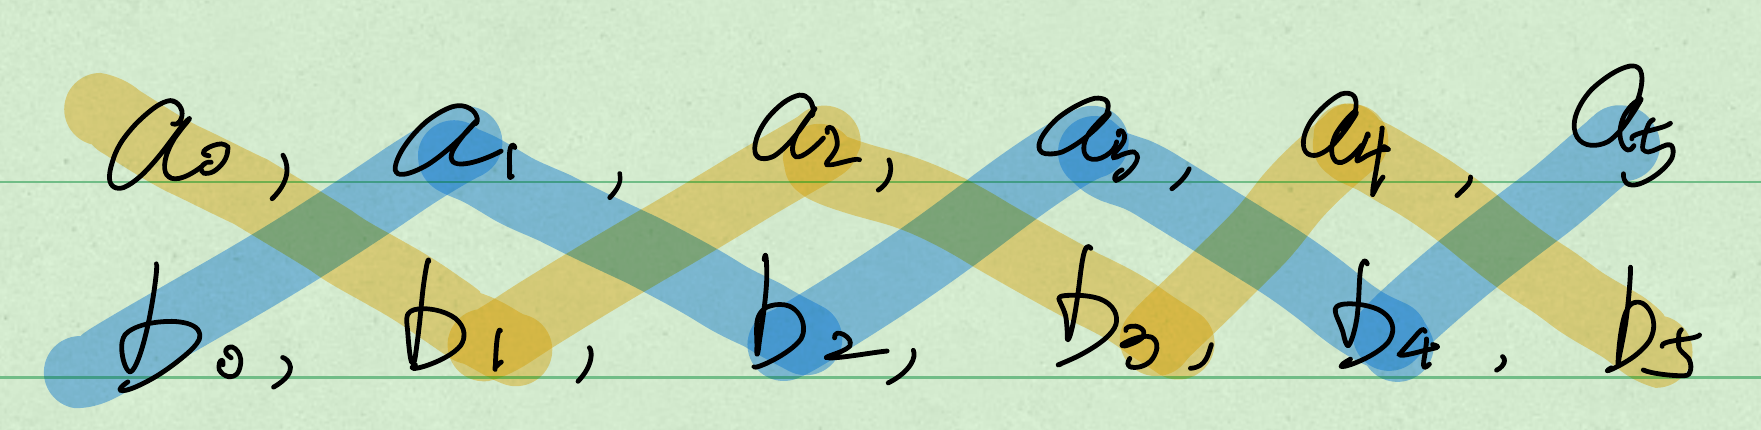
\includegraphics[width=0.6\textwidth]{merging-two-sorted-lists}}

This specific claim lists $2n-1$ comparisons and hence
would prove the lower bound. But the adversary should give a consistent
set of answers.
\end{proof}
\item \emph{{[}!{]} The algorithm which compare $b_{i}$ with $a_{i}$ as
well as $a_{i+1}$ is rather intuitive. How does it come? Why we
have the confident to say it is the lower bound, in other words, best
of the best?}
\begin{proof}
Suppose the algorithm fails to perform the comparison $b_{i}$ with
$a_{i}$ for some $i$. Then both of the following orders are consistent
with all of the adversary answers:
\begin{align*}
a_{1}<b_{1}<a_{2}<\cdots<a_{i-1}<b_{i-1}<\boldsymbol{a_{i}<b_{i}}<\cdots<b_{n}\\
a_{1}<b_{1}<a_{2}<\cdots<a_{i-1}<b_{i-1}<\boldsymbol{b_{i}<a_{i}}<\cdots<b_{n}
\end{align*}
 Thus the algorithm cannot know which of these two orders is correct
and hence cannot stop. Similarly we can show that if any comparison
of $b_{i}$ with $a_{i+1}$ is not performed by the algorithm, again
there are at least $2$ possible orderings consistent with all the
answers obtained so far. 
\end{proof}
\item You may have noticed that although we have couched the last argument
as an adversary argument, the adversary does not really adapt to the
questions asked by the algorithm. The worst-case input that she produces
is the same for all algorithms! Nevertheless, the adversary argument
provides greater clarity especially emphasizing the point that if
the algorithm decides to output one of two surviving orderings at
the end, the adversary can always arrange for the correct order to
be the other one. 
\end{itemize}
\end{itemize}

\paragraph*{Connectivity}

An undirected graph is connected when it has at least one vertex and
there is a path between every pair of vertices. Equivalently, a graph
is connected when it has exactly one connected component. In a connected
graph, there are no unreachable vertices. An undirected graph that
is not connected is called disconnected. An undirected graph G is
therefore disconnected if there exist two vertices in G such that
no path in G has these vertices as endpoints. The below graph becomes
disconnected when the dashed edge is removed.

\centerline{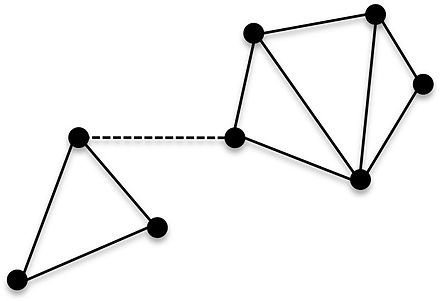
\includegraphics[width=0.5\textwidth]{Sample-graph}}

\paragraph*{Adversary Lower Bounds in the Edge Probe Model}

You are given the vertex set $V$ of a graph, but its edges are initially
unknown. In the edge probe model the algorithm is allowed to query
any pair of vertices $(i,j)$ and learns whether there is an edge
between $i$ and $j$. The algorithm needs to determine whether the
graph has some property. 

For example, let us imagine that the goal of the algorithm is to determine
\textbf{if the graph is connected}. The model of computation here
counts the number of edge probes made by the algorithm. A \textbf{trivial
upper bound} is $\binom{n}{2}$, since the algorithm can query 
all
pairs, determine the entire graph, and then easily decide if it is
connected. 

To give a lower bound, we imagine an adversary answering the probes
made by the algorithm and design a strategy for the adversary to answer
these probes to make the algorithm take as many steps as possible.
A naive first attempt might be to suggest that the adversary keeps
saying \textquotedblleft no\textquotedblright{} to each edge probe.
But then the algorithm that first probes all $n-1$ pairs involving
the vertex $1$, would conclude in $n-1$ probes that the graph is
not connected, because vertex $1$ is isolated. 

Likewise answering ``yes\textquotedblright{} to every edge probe
does not work since an algorithm can find a spanning tree in just
n \textminus{} 1 probes. Thus, in order to create a difficult graph
the adversary must judiciously mix \textquotedblright yes\textquotedblright{}
and \textquotedblright no\textquotedblright{} answers. A good adversary
strategy is the following:

\emph{Playing against any algorithm, the adversary maintains the connected
components in the graph formed by the edges the algorithm has discovered
already. Now when the algorithm makes the probe $(i,j)$, the adversary
answers \textquotedblright yes\textquotedblright{} if and only if
$(i,j)$ is the last possible edge connecting the component of $i$with
the component of $j$. }

In other words, if A says ``Yes, there is an edge between i and j'',
it means\emph{ i is the only vertex connects to j and A has checked
every vertex with j except i.}

If the algorithm does not make all $\binom{n}{2}$ probes, the 
graph
will be disconnected, with the possibility of becoming connected if
the unprobed pairs are revealed to be edges. Thus the algorithm will
be unable to stop and correctly determine if the graph is connected.
How do we prove this? We do so by proving the following statements: 
\begin{lemma}
For any algorithm A, at any stage, let C be a connected component
that has been revealed by the probes that A has made. Then A must
have probed every pair of distinct vertices in C, which cost $\binom{n}{2}$
steps.
\end{lemma}
\begin{proof}
\emph{We prove checking connectivity cost $\binom{n}{2}$ steps by
induction}. 

Base case, the number of probe has been executed is 0. Initially no
edges have been discovered, each component is a singleton vertex,
and it is vacuously true that every pair of distinct vertices in any
component has been probed. 

Inductive hypothesis, suppose after the algorithm makes its i-th probe,
the graph is connected.

We want to show that the graph is still connected after the (i+1)-th
probe. Say this probe is the pair $(u,v)$. If this probe gets the
answer \textquotedblright no\textquotedblright , then no edges are
added and the connected components remain the same. Hence the inductive
hypothesis ``carries over\textquotedblright{} and all pairs in each
component have been probed as before. 

If on the other hand, suppose the pair $(u,v)$ is revealed to be
an edge. Now a new connected component is formed merging together
the components of $u$ and $v$. Have all pairs of vertices in this
component been probed? By the inductive hypothesis every pair within
the component of u and within the component of v (before edge $(u,v)$
was added) must have been probed. By the adversary strategy, all pairs
between vertices in these two components must have already been probed
for the adversary to answer yes. Thus all pairs within the new component
containing u and v must have been probed, and the inductive proof
is complete. 
\end{proof}
\begin{lemma}
If the algorithm proceeds to probe all pairs, it will discover that
the graph is connected. 
\end{lemma}
\begin{proof}
This is easy to see from the adversary strategy. The aim of the adversary
is, suppose there is a connected graph with n vertex, trying to make
the graph so that edge detecting algorithm could discover the connectivity
as late as possible.
\end{proof}

\subsection{Conclusions }

This handout presents a far rosier picture of lower bound theory than
is true. In fact non-trivial lower bounds are practically unknown
on general computational models like the computers you use. The best
lower bounds are obtained when restricted models of computing such
as the comparison tree model are considered. Even here there is not
an abundance of general techniques. Proving a lower bound for a particular
problem usually calls for a good deal of ingenuity and perseverance.
The edge probe model has been widely studied. Properties such as connectivity
that require an algorithm to probe all possible pairs are said to
be \textbf{evasive}. It turns out that many interesting properties
are evasive, and there are many beautiful results that show that a
large class of properties are evasive. 

\part{Algorithm Design and Analysis Paradigms}

\section{Recurrence Relation}

\section{Quick Sort}
\begin{itemize}
\item Input: Array of $n$integers.
\item Outputs: These integers in certain order.
\end{itemize}

\subsection{Algorithm:}
\begin{itemize}
\item Pick an element $x$as the pivot element
\item By comparing each of the elements with the pivot, place it in one
of the two sets:
\begin{align*}
 S=\{y:y<x\}\\
 L=\{y:y>x\}
\end{align*}
\item Recursively sort $S$ and $L$.
\item Output $S\times L$.
\end{itemize}

\subsection{Performance:}
\subsubsection{Worst Case}
Each partition routine produces one sub-problem with n-1 elements and one with 
0 elements.
\begin{align*}
 T(n)&\ge\Theta(n)+T(n-1)
 &\intertext{Based on substitution method,}
 T(n)&=\Theta(n^{2})
\end{align*}
\subsubsection{Expected Running Time}
Calculate the expected number of comparison made by QuickSort in the worst 
case when the pivot is selected randomly.
\begin{itemize}
\item Algorithm: pick pivot uniformly of random from the elements to be
sorted.
\item Analysis:
\begin{itemize}
\item Let $x$ be the total amount of comparison are formed by QuickSort. 
\item Let $x_{ij}$ be a random variable that is : 

$$x_{ij}=
\begin{cases}
1 & \text{if i-th smallest element and j-th smallest element are compared.}\\
0 & \text{otherwise.}
\end{cases}
$$
\item $x=\sum_{i<j}x_{ij}$
\item $E[x]=E[\sum_{i<j}x_{ij}]=\sum_{i<j}E[x_{ij}]$ (Linearity of Expectation)
$=\sum_{i<j}Pr[x_{ij}=1]$
\item $x_{i}$ and $x_{j}$ are compared if and only if the firs element
to be chosen as a pivot from $x_{ij}$ is either $x_{i}$ or $x_{j}$.
\item Pr\{$z_{i}$ is compared to $z_{j}$\} = $\frac{2}{j-i+1}$
\end{itemize}
\item 
Expectated 
Running time
\begin{align*}
 E[x]&=\sum_{i<j}Pr[x_{ij}=1]
 =\sum_{i<j}\frac{2}{j-1+1}\\
 &=\sum_{i<j} \frac { 2 } { k+1 }\\
 &<\sum_{i=1}^{n-1}\sum_{j=i+1}^{n}\frac{2}{k}\\
 &=\sum_{i=1}^{n-1}O(\log n)=O(n\log n)
\end{align*}
\end{itemize}

\section{Selection/ order}
\begin{itemize}
\item Input: A set of $A$ of n integers and a rank $i$, with $1\ge i\ge n$.
\item output: The element $x\in A$ that is larger than exactly $i-1$ other
elements of $A$.
\end{itemize}
We can solve the selection problem in $O(n\log n)$ time since we
can sort the number using heapsort or mergesort and then simply index
the $i$-th element in the output array. But we can do better than this.

\subsection{Randomized-Select}
\begin{algorithm}[H]
    \SetKwProg{Fn}{Function}{:}{}
    \SetKwFunction{FRandSelect}{RANDOMIZED-SELECT}
    \SetKwFunction{FRandPartition}{RANDOMIZED-PARTITION}

    \Fn{\FRandSelect ($A, p, r, i$)}{
%         \KwData{Array $A[p, \cdots, r]$, rank $i$}
        \uIf{p == r}{
            return A[p]
        }
        q = \FRandPartition(A, p, r){}
        
        k = q - p + 1 
        
        \uIf {i == k}{\tcc{The pivot is the answer}
            return A[q]
        }
        \uElseIf {i < k}{
            return \FRandSelect ($A, p, q-1, i$)
        }
        \Else{
            return \FRandSelect ($A, q+1, r, i-k$)
        }

    }
 \caption{Randomized-Select}
\end{algorithm}
The worst-case running time for RANDOMIZED-SELECT is $\Theta(n^2)$, because we 
could be extremly unlucky and always parition around the largst remaining 
element, and the parition takes $\Theta(n)$ times.

But the algorithm has a linear expected running time $O(n)$, and because it is 
randomized, no particular input elicits the worst-case behavior.
\subsection{Deterministic Linear Time Selection}
After quick selection, algorists looked for an angorithm which is able to solve 
the problem in linear deterministicly.

\centerline{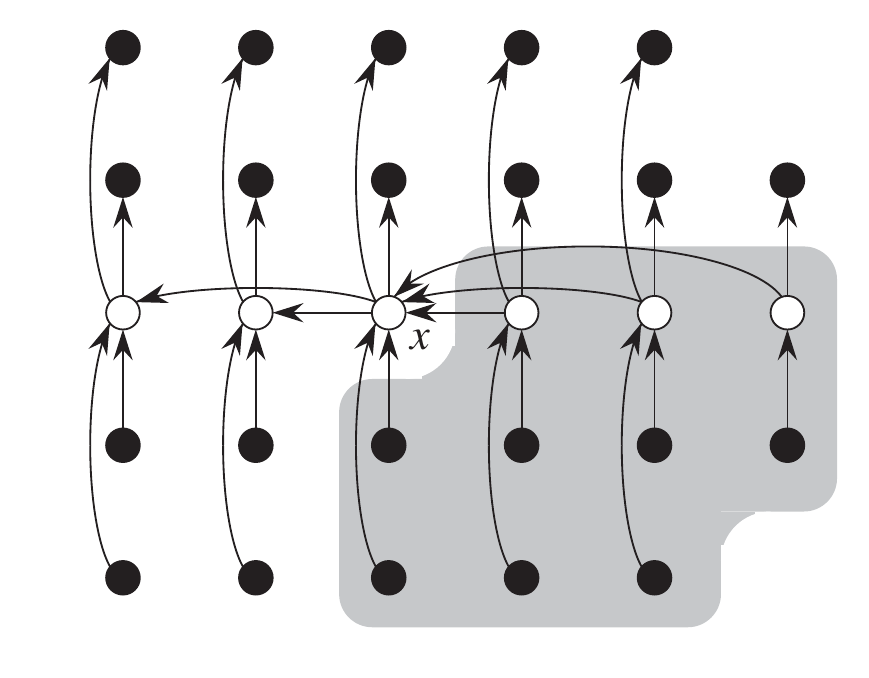
\includegraphics[width=0.5\textwidth]{deterministic-select.png}}

SELECT Algorihtm:
\begin{itemize}
\item Find the medium of each group by insertion-sorting. $T(n) = \frac{6n}{5} 
= 1.2n$.
\item Use SELECT to recursively find the medium of the mediums $m^*$.
\item $m^*$ has a rank somewhere in the middle.
We treat the median of the medians $m^*$ as a pivot element and compare all 
elements, which takes $n$ steps.
    \begin{itemize}
        \item The number of elements larger than $m^*$: $O(\frac{3n}{10}) 
    =3(\ceil*{\frac{1}{2}\ceil*{\frac{n}{5}} - 2})$
        \item Therefore, the number of element smaller than $m^*$: 
    $O(\frac{7n}{10})$.
    \end{itemize}
\item Pivot using $m^*$:
    \begin{itemize}
     \item If $i = k$, then return $k$.
     \item If $i < k$, use SELECT recursively to find the $i$-th smallest 
element on the low side.
     \item If $i > k$, use SELECT recursively to find the $(i-k)$-th smallest 
element on the high side.
    \end{itemize}
\end{itemize}
Therefore, the recursion of the algorithm is
\[T(n) \le T(\frac{n}{5}) + T(\frac{7n}{10}) + 2.2n\]
We guess $T(n) \le cn$ and it can be proved by induction.
\begin{itemize}
\item Base case:
    \begin{align*}
    T(\frac{n}{5}) &\le \frac{cn}{5}\\
    T(\frac{7n}{10}) &\le \frac{c7n}{10}
    \end{align*}
\item hypothesis: $T(n) \le \frac{cn}{5} + \frac{c7n}{10} + 2.2n$
\item Inductive step:
    \begin{align*}
    cn &\ge \frac{cn}{5} + \frac{c7n}{10} + 2.2n\\
    10 cn &\ge 2cn + 7cn + 22n\\
    c &\ge 22
    \end{align*}

\end{itemize}




\part{Graph Algorithms}

\part{NP-completeness}

\part{Approximation Algorithms}

\part{Randomized Algorithms}.

\end{document}
